\documentclass{book}

% external files
%% util
% set paragraph distance
\setlength{\parskip}{0.7em}
\parindent 0em

\usepackage[BoldFont, SlantFont, CJKchecksingle]{xeCJK}
\usepackage{fontspec}
\usepackage[xetex, unicode=true,
  bookmarksnumbered, bookmarksopen,
  colorlinks=true, citecolor=green,
  linkcolor=blue, pdfcreator={coanor},
  urlcolor=blue]{hyperref}

% Make `` '' and `' works well under xelatex 
\defaultfontfeatures{Mapping=tex-text}

\usepackage[toc,page]{appendix}

% various labels
\usepackage{bbding}

% geometry
%\usepackage[a6paper, left=0.2cm,top=0.5cm,right=0.2cm,bottom=0.5cm,bindingoffset=0.5cm]{geometry}
%\usepackage[a6paper, left=5mm,top=0.5cm,right=7mm,bottom=0.5cm]{geometry}
%\usepackage[a4paper, left=5mm,top=0.5cm,right=5mm,bottom=0.5cm]{geometry}
%\usepackage{geometry}

% page head/foot, disable them while output to Kindle format
%\usepackage{fancyhdr}
%\pagestyle{fancy}
%\fancyhf{}
%\fancyhead[RE]{\footnotesize\textit{\nouppercase{\leftmark}}}
%\fancyhead[LO]{\footnotesize\textit{\nouppercase{\rightmark}}}
%
%\fancypagestyle{plain} {
%	\fancyhf{}
%	\renewcommand{\headrulewidth}{0pt}
%	\renewcommand{\footrulewidth}{0pt}
%}

\usepackage{amsmath}

% inline list
\usepackage{paralist}

% images
\usepackage{graphicx}
\usepackage{sidecap}
\usepackage[english]{babel}
\usepackage{wrapfig}
\usepackage{subcaption}

\usepackage[normalem]{ulem}

\usepackage[hypcap]{caption}

\usepackage{hhline} 
\usepackage{array} 
\usepackage{pbox} 

\usepackage{pdftexcmds}
\usepackage{catchfile}
\usepackage{ifluatex}
\usepackage{ifplatform}
\iflinux
\setCJKmainfont{PMingLiU}
%\setCJKmainfont{SimSun}
%\setCJKmainfont{NSimSong}
%\setmainfont{Century Schoolbook L}
%\setmainfont{Plantagenet Cherokee}
%\setmathfont{Latin Modern Math}
%\setmonofont{Nimbus Mono L:style=Bold}
\setmonofont{Courier New}
%\setmonofont{TlwgMono:style=Bold}
%\setmonofont{DejaVu Sans Mono:style=Book}
\fi

\ifwindows
\setCJKmainfont[BoldFont=SimHei]{SimSun}
\setCJKmonofont{SimSun} % defaul chinese font
%\setmainfont{Cambria}
%\setmonofont{Inconsolata}
%\setmathrm{Cambria Math}
%\setsansfont{Calibri}
\fi

\ifmacosx
\setCJKmainfont[BoldFont=SimHei]{SimSun}
%\setCJKmonofont{STFangsong} % defaul chinese font
%\setCJKmainfont{PMingLiU}
\setCJKmainfont{Songti TC}
\setmonofont{Menlo}
%\setmainfont{Apple Chancery} % beauty
%\setmainfont{PilGi} % beauty but can not reading...
%\setmainfont{Futura}
\fi

\usepackage[tikz]{bclogo}
\usepackage{listings}
\definecolor{dkgreen}{rgb}{0,0.6,0}
\definecolor{gray}{rgb}{0.5,0.5,0.5}
\definecolor{mauve}{rgb}{0.78,0,0.42}
\definecolor{light-gray}{gray}{0.8}

\newcommand{\codefs}{\scriptsize}

% out put font
\newcommand{\outputf}{\itshape\codefs}
\newcommand{\inputf}{\slshape\codefs}
\newcommand{\cf}{\ttfamily\small}
% hight light text
\newcommand{\hl}[2]{\color{#1}{\ttfamily\scriptsize #2}}

\usepackage{caption}
\usepackage{listings}

\DeclareCaptionFont{white}{ \color{white} }
\DeclareCaptionFormat{listing}{
    \colorbox[cmyk]{0.43, 0.35, 0.35,0.01 }{
        \parbox{\textwidth}{\hspace{15pt}#1#2#3}
    }
}

\captionsetup[lstlisting]{format=listing, labelfont=white, textfont=white, singlelinecheck=false, margin=0pt, font={bf,scriptsize}}

\lstset{
	language=C, % the language of the code
	basicstyle=\ttfamily\scriptsize, % the size of the fonts that are used for the code
	%numbers=left, % where to put the line-numbers
	%numberstyle=\tiny\color{gray}, % the style that is used for the line-numbers
	%stepnumber=1, % the step between two line-numbers. If it's 1, each line will be numbered
	%numbersep=8pt, % how far the line-numbers are from the code
	%backgroundcolor=\color{light-gray}, % choose the background color. You must add \usepackage{color}
	backgroundcolor=\color{white}, % choose the background color. You must add \usepackage{color}
	showspaces=false, % show spaces adding particular underscores
	showstringspaces=false, % underline spaces within strings
	showtabs=false, % show tabs within strings adding particular underscores
	%
	% adds a frame around the code
	%
	%frameround=fttt,
	%frame=trBL,
	%framexleftmargin=2mm,
	%frame=trbl,
	%frameshape={RYRYNYYYY}{yny}{yny}{RYRYNYYYY},
	%rulesepcolor=\color{blue},
	rulecolor=\color{black}, % if not set, the frame-color may be changed on line-breaks within not-black text (e.g. commens (green here))
	tabsize=2, % sets default tabsize to 4 spaces
	%captionpos=b, % sets the caption-position to bottom
	breaklines=false, % sets automatic line breaking
	breakatwhitespace=true, % sets if automatic breaks should only happen at whitespace
    %title={\it \lstname}, % show the filename of files included with \lstinputlisting; also try caption instead of title
	keywordstyle=\bfseries\color{green!40!black}, % keyword style
	commentstyle=\itshape\color{purple!40!black}, % comment style
	stringstyle=\color{mauve}, % string literal style
	escapeinside=\`\`, % if you want to add LaTeX within your code
	morekeywords={*,restrict,...}, % if you want to add more keywords to the set
	linewidth=0.99\textwidth,
	xleftmargin=0.5cm,
	%identifierstyle=\color{blue},
}

\input{../input/more-key} 

% add new font
\newfontfamily{\lc}[Scale=MatchLowercase]{Verdana}
\newfontfamily{\uc}[Scale=MatchUppercase]{Arial}

%\newcommand{\cf}{\footnotesize\tt}
\newcommand{\lcf}{\small\tt}
\newcommand{\fem}{\footnotesize\em}
\newcommand{\fsf}{\footnotesize\sf}
\newcommand{\hsf}{\huge\sf}
\newcommand{\hbf}{\Huge\bf}
\newcommand{\fit}{\footnotesize\it\hfill}
% emph font
\newcommand{\ef}{\it\uc}
% reference font
\newcommand{\rf}{\footnotesize\lc}
% new word font
\newcommand{\nf}{\sf}
% section font
\newcommand{\secf}{\normalsize\sf}
% file name font
\newcommand{\ff}{\scriptsize\lc}
% cf in chinese env
\newcommand{\ccf}{\footnotesize\tt\color{magenta}~}
% font for commands
\newcommand{\cmdf}{\footnotesize\sf}
% font for caption
\newcommand{\capf}{\footnotesize\lc}
% string in code
\newcommand{\str}[1]{``{\footnotesize #1}''}

% marginpar redefinition
\newcommand{\fmp}[1]{\marginpar{\scriptsize #1}}

% important words
\newcommand{\iw}[1]{\uwave{#1}}
\newcommand{\bif}[1]{\textbf{\textit{#1}}}

\newcommand{\hreff}[1]{\small\bfseries\sffamily{#1}}

% URL reference
%\newcommand{\uref}[2]{\href{#1}{\small\bfseries\textsl{#2}}}
\newcommand{\uref}[2]{\href{#1}{\small\sffamily{#2}}}

% table column font
\newcommand{\tcf}{\scriptsize}

%\makeatletter
%\renewcommand\@seccntformat[1]{\secf}
%\makeatother

\usepackage{titlesec}
%\titleformat*{\section}{\normalsize\bfseries\sffamily\color{blue}}
%\titleformat*{\subsection}{\small\bfseries\sffamily\color{blue}}
%\titleformat*{\subsubsection}{\footnotesize\bfseries\sffamily\color{blue}}
\titleformat*{\section}{\bfseries\sffamily\color{blue}}
\titleformat*{\subsection}{\bfseries\sffamily\color{blue}}
\titleformat*{\subsubsection}{\bfseries\sffamily\color{blue}}


\title{\hsf 数据库防火墙 Suricata 开发文档}
\author{tanb}
\date{Apr 22, 2014}

\begin{document}

\maketitle

\begin{table}[!h]
    \centering
    \caption{文档更新历史}
    \begin{tabular}{|>{\scriptsize}r|>{\scriptsize}r|>{\scriptsize}p{6cm}|} \hline
        日期        & 作者 & 详情    \\ \hline\hline
        May 4, 2014 & tanb & 加入 \ref{sec:12c-tns} 节;修正之前的一些描述错误 \\\hline
        May 6, 2014 & tanb & 加入 \ref{sec:dev-problems} 节; \\\hline
        Jun 3, 2014 & tanb & 更正一些描述错误 \\\hline
        Jun 6, 2014 & tanb & 加人 demo(\ref{chap:demo}) 章节 \\\hline
        Jun 17, 2014 & tanb & 修正 Oracle 协议中超长字符串的描述(\ref{sec:oracle-query-string}) \\\hline
    \end{tabular}
    \label{tab:update-hist}
\end{table}

\tableofcontents

\chapter{数据库环境的准备}
本章主要记录如何准备各种目标数据库,其中着重记录了 Oracle 11g R2 的安装以及配置。因为它总是如此让人捉摸不透。

\section{Oracle 11g R2 环境的安装和使用}
近期可获取的 Oracle 的最老版本为 11g R2,安装之前可以先去 Oracle 官网下载该版本的数据库。

准备条件:\footnote{本节中的内容全部在 Linux 环境,不考虑 Windows 的兼容性。}

\begin{itemize}
\item 一个带桌面环境的 Linux 发行版,将其作为宿主机器,你需要它的 X 环境来点击 Oracle 安装过程中的各种按钮。
    %\begin{quote}
    %    when install oracle in Centos, you may need to install X11:
    %        
    %    \begin{lstlisting}
    %        yum groupinstall basic-desktop desktop-platform x11 fonts
    %    \end{lstlisting}

    %    Then edit {\ff /etc/inittab}, change {\cf id:3:initdefault:} to {\cf id:5:initdefault:} to start X at boot-up
    %\end{quote}

\item Oracle 专用的 Linux 发行版,推荐 {\ff OracleLinux-R6-U5-Server-x86\_64-dvd.iso},如果需要其它版本,到\href{http://mirrors.wimmekes.net/pub/iso/}{这里}下载。

\item Oracle 11g R2,到 Oracle 官网下载两个文件 {\ff linux.x64\_11gR2\_database\_1of2.zip} 和 {\ff linux.x64\_11gR2\_database\_2of2.zip}。

\item Oracle 的 instant client,到 Oracle 官网下载 {\ff instantclient-basic-linux-12.1.0.1.0.zip} 和 {\ff instantclient-sqlplus-linux-12.1.0.1.0.zip}。\footnote{我下载的大版本号是 12,其实它是兼容服务器端的 11 版本号。如果碰到问题,请直接下载其版本为 11 的客户端。}
\end{itemize}

如果没有实体机器,就用 Virtualbox 虚拟几个,一个用于安装 Oracle Linux,一个用于安装客户端,客户端推荐使用 Linux,可以用 Ubuntu,为节约性能,直接使用不带 UI 的 Ubuntu 即可,如 {\ff ubuntu-12.04.4-server-amd64.iso};但对服务器端而言,最好选择 Oracle 自己的 Linux 发行版,其它版本的 Linux 虽然也可以安装 Oracle,但说多了都是泪,直接用 Oracle 自己的 Linux 发行版是最好的选择。

在 Virtualbox 中安装这两个 Linux 系统,如果可以,将服务器的内存尽量放大一点(2G+)。安装完后,将两个虚拟机的 IP 设置为桥接模式,重启网络后\footnote{\cf /etc/init.d/network restart},这样它们与宿主机就处于同一网段,假定 Oracle Linux 的 IP 为 {\cf 192.168.37.194},Ubuntu 客户机的 IP 为 {\cf 192.168.37.193}。

\begin{quote}
有时候安装的 Oracle Linux 只能使用环回地址(lo),用 {\cmdf ifconfig -a} 查看后,确实有 {\cf eth0},此时需要启动一下该网卡,并设置其通过 DHCP 获取 IP 地址。

    \begin{lstlisting}
    ifconfig eth0 up
    # 在 /etc/sysconfig/network-scripts/ifcfg-eth0 中
    DEVICE=eth0
    BOOTPROTO=dhcp
    ONBOOT=yes
    # 然后重新启动 eth0
    ifup eth0
    \end{lstlisting}

\end{quote}

接下来将下载的 Oracle 数据库安装文件拷贝到 194,将 instantclient 拷贝到 193。分别以 SSH 登录到这两台机器。

\begin{lstlisting}
xhost +192.168.37.194 # 设定 X 服务,使得 194 可以访问 host 上的 X 服务
ssh -X 192.168.37.194
ssh -X 192.168.37.193
\end{lstlisting}

由于两个虚拟机都不带桌面环境,所以此处用 {\cf -X} 选项,使得它们可以访问宿主机上的桌面环境。

在 Oracle Linux 上安装 Oracle 11g R2,参见\href{http://www.oracle-base.com/articles/11g/oracle-db-11gr2-installation-on-oracle-linux-6.php}{这里}的详细步骤。

然后安装客户端,将两个 zip 文件解压后,会得到目录 {\ff instantclient\_12\_1},然后设置两个环境变量 {\cf PATH} 和 {\cf LD\_LIBRARY\_PATH},将它们指向该目录。

接下来在 {\cf instantclient\_12\_1} 中,编辑两个文件。第一个为 {\ff sqlnet.ora},在其中加入如下内容

\begin{lstlisting}
QLNET.AUTHENTICATION_SERVICES= (NTS)
NAMES.DIRECTORY_PATH= (TNSNAMES, EZCONNECT)
\end{lstlisting}

第二个文件为 {\ff tnsnames.ora},在其中加入如下内容

\begin{lstlisting}
databasename =
(DESCRIPTION =
 (ADDRESS_LIST =
  (ADDRESS = (PROTOCOL = TCP)(HOST = 192.168.37.194)(PORT = 1521))
 )
 (CONNECT_DATA =
  (SERVICE_NAME = orcl11g)
 )
 )
\end{lstlisting}

为便于连接 194 上的数据库,编写脚本 {\ff login-oracle.sh}:

\begin{lstlisting}
sqlplus system/test@'(DESCRIPTION=(ADDRESS=(PROTOCOL=TCP) \
  (HOST=192.168.37.194)(PORT=1521))(CONNECT_DATA=(SID=orcl11g)))'
\end{lstlisting}

客户端配置完毕,此时你应该可以在命令行执行该登录脚本。但是登录不会成功。

接下来配置服务器端,由于 Oracle Linux 默认开启了多个 iptables 的防火墙设置,所以需要将它们一一关闭,登录 194:

\begin{lstlisting}
service iptables save
service iptables stop
chkconfig iptables off

service ip6tables save
service ip6tables stop
chkconfig ip6tables off
\end{lstlisting}

这样,在 193 上应该就能访问 194 上的服务了。

当下一次服务器重启的时候,可能你什么都找不到了,但是没关系,上面的链接中给了很多设定,最重要的是环境变量,没记错的话,应该都放到用户目录的 {\ff .bash\_profile} 中去了。如果下一次启动的时候,这些环境变量都没了(典型的表现是输入 {\cmdf sqlplus} 说找不到这个命令),那么在命令行执行

\begin{lstlisting}
source .bash_profile
\end{lstlisting}

即可,这样所有的环境变量又会来了。接下来启动 Oracle 数据库服务器:

\begin{lstlisting}[language=sh]
dbstart &
\end{lstlisting}

执行上面的登陆脚本,此时应该就能正常登入了。

登陆进入 Oracle 数据库之后,可以用如下 SQL 语句,以测试数据包的抓取:

\begin{lstlisting}[language=sql]
SELECT owner, table_name FROM dba_tables;
SELECT table_name FROM all_tables;
SELECT * FROM information_schema.columns WHERE table_name = 'abc';
SELECT DISTINCT OWNER FROM ALL_OBJECTS;

SELECT * from all_users; -- 列出所有用户
SELECT table_name FROM all_tables; -- 列出用户所能访问的表
SELECT * FROM all_tables; -- 列出用户所能访问的表
SELECT UTL_INADDR.get_host_address from dual; -- 列出当前登录的 server IP
\end{lstlisting}
%SELECT name from v$database;    -- 列出所有的数据库(需 system 用户登录)

\section{Mysql 环境的安装和使用}
这个比较简单,是个 Linux 都能跑 Mysql,以 Ubuntu 为例,直接在源中安装 mysql 即可。客户端也可以从源中安装。对于出现的错误,网上都有例子,以错误代码 Google 即可。不表。

\section{DB2 环境以及 SQL Server 的安装和使用}
DB2 和 SQL Server 的环境都比较好安装。 DB2 分别提供了 Linux 和 Windows 的安装镜像。SQL Server 目前的版本为 SQL Server 2012,也可以去渣软的官网下载。其安装和使用也比较简单,此处不表。

\subsection{SQL Server 2012 的配置}
SQL Server 2012 的安装比较简单,各种「下一步」即可。这里主要记录一下如何配置服务器,让其可以外部访问。

这里先假定安装过程中指定了 {\cf SQL Server Authentication} 选项,不然难以从远程登陆。如果指定了该选项,则用户名为 {\cf SA}。此外,假定你创建的实例名称为 {\cf DEVDB}(默认为 {\cf MSSQLSERVER} 或 {\cf SQLEXPRESS})。

安装完成过后,打开开始菜单中的 {\cf Microsoft SQL Server 2012 -> Configuration Tools -> SQL Server Configuration Manager}。进入左边的 {\cf SQL Server Network Configuration -> Protocols for DEVDB},在右边的列表中,选择 {\cf TCP/IP},右键进入 {\cf Properties},进入 {\cf IP Addresses} 列表,拖到最后的 {\cf IPAll},将 {\cf TCP Port} 设置为 1433,应用之。

然后在左边列表中选择 {\cf SQL Server Services},重启对应的 {\cf SQL Server(DEVDB)},使之生效。

这样,用开始菜单中的 {\cf SQL Server Management Studio} 做一下测试,连接本机的服务器。假定服务器 IP 为 {\cf 192.168.37.160},在弹出的 {\cf Connect to Server} 对话框中,做如下设置:

\begin{itemize}
    \item {\cf Server type}: 选择 {\cf Database Engin}
    \item {\cf Server name}: {\cf 192.168.37.160}
    \item {\cf Authentication}: 选择 {\cf SQL Server Authentication}
    \item {\cf Login}: 用 {\cf SA} 登陆
    \item {\cf Password}: 自己填
    \item 选择 {\cf Options},进入选项设置
    \item {\cf Connect to database}: 手动填写 {\cf DEVDB}
    \item {\cf Network protocol}: 选择 {\cf TCP/IP}
    \item 点击连接
\end{itemize}

此时应该可以连接到服务器了。

在 Linux 中,直接用 {\cmdf tsql} 连接服务器:

\begin{lstlisting}
    tsql -S 192.168.37.160 -U sa
\end{lstlisting}

需要注意的是,事先检查一下 {\cmdf tsql} 编译时指定的 TDS 版本号。经测试 SQL Server 2012 不支持默认的 TDS 5.0 版本,需要编译时手动指定 7.0 版本。

在 {\cmdf tsql} 中执行 SQL 语句时,需要用 {\cf go} 指令:

\begin{lstlisting}
    1> select * from sys.tables
    2> go
\end{lstlisting}

去 Wireshark 中抓包吧。

\section{如何用 Wireshark 抓取数据包}
本节主要讲述如何用 Wireshark 抓取数据包,由于要展现全貌,为便于排版,图片比较小,可放大查看。

以 Oracle 的 TNS 协议为例,下面演示了如何在 Wireshark 中抓取通信数据包的过程。

在 Linux 下,以 root 启动 Wireshark ,设置一下侦听的网卡后即可抓取数据包。但是如果需要抓取特定协议的数据包,可以在 {\ef Filter} 中输入过滤条件,以 TNS 协议为例,其设置如图 \ref{fig:wireshark-tns} 所示:

\begin{figure}[ht!]
    \caption{Wireshark 抓取的 Oracle 数据包示例}
    \label{fig:wireshark-tns}
    \centering
    \includegraphics[width=\textwidth]{wireshark-tns.png}
\end{figure}

此处的过滤规则为 {\cf tns and ip.addr==192.168.37.194},其实,只要第一条即可,它限定了只显示与 TNS 协议相关的数据包。

图上列举的数据包中,来自一个 Oracle 的登陆操作。其中 174 作为客户端,194 作为服务器端,在第一条数据包中,{\ef Length} 列列出了数据包长度,{\ef Info} 列列出了是该数据包的详细信息,其中 {\cf Request} 指客户端请求服务器端,{\cf (1)} 是数据包类型,此处指一个 {\cf Connect} 操作。

在这条数据包中,从右下角的报文中可以看出,其中包含着一个 TNS 连接字符串,在该字符串中列举了连接的实例名 {\cf SID}、客户端工具为 {\cf sqlplus},客户端的主机名,使用的通信协议(TCP),客户端的 IP 以及连接的服务器端的端口。

左下角即是具体的数据包分析,Wireshark 目前只能识别部分 TNS 协议,比如连接数据包,对其他数据包,则只能识别头部数据,数据包后面的数据则不能识别。

对客户端发送出来的连接数据包而言,其中列举了包长度、校验和、包类型等等,图 \ref{fig:tns-connect} 中列出了 Wireshark 所分析出来的登陆数据包:

\begin{figure}[h!]
    \caption{Oracle 客户端发出的连接数据包}
    \label{fig:tns-connect}
    \centering
    \includegraphics[width=\textwidth]{tns-connect.png}
\end{figure}

如果验证通过,服务器端会返回其 {\cf Accept} 数据包,Wireshark 的分析结果如图 \ref{fig:tns-accept} 所示:

\begin{figure}[h!]
    \caption{Oracle 服务器端发出的 Accept 数据包}
    \label{fig:tns-accept}
    \centering
    \includegraphics[width=0.8\textwidth]{tns-accept.png}
\end{figure}

连接建立以后,就可以发送 SQL 请求给服务器端,以下面的 SQL 语句为例:

\begin{lstlisting}[language=sql]
SELECT table_name FROM all_tables;
\end{lstlisting}

其 Wireshark 的分析结果如图 \ref{fig:tns-select} 所示:

\begin{figure}[h!]
    \caption{Oracle 的 SQL 查询语句数据包}
    \label{fig:tns-select}
    \centering
    \includegraphics[width=\textwidth]{tns-select2.png}
\end{figure}

从右下角的报文可以看出,其中就包含有查询语句,但是从左下角 Wireshark 的报文分析来看,它并没有识别出该报文。而且经测试,同一条 SQL 语句,其报文结构{\bf 可能}不同,比如,再次输入上面的 SQL 语句,其报文如图 \ref{fig:tns-select-diff} 所示,此处再次列出上面的图片以做对比。\footnote{这种不同是有规律的,登陆后第一条查询语句的 payload 首字节为 {\cf 0x035e},后续的查询都是以 {\cf 0x1169}
开头,后面相隔固定字符之后再追加 {\cf 0x035e}。}

\begin{figure}[ht!]
    \caption{Oracle 中同一条 SQL 查询语句出来的数据包可能不同}
    \label{fig:tns-select-diff}
    \centering
    \includegraphics[width=\textwidth]{tns-select.png}
    \includegraphics[width=\textwidth]{tns-select2.png}
\end{figure}

以上是 Oracle 数据库通信协议的 Wireshark 截图。下面再用 Wireshark 分析一下 MySQL 的通信数据包。

在 MySQL 的客户端与服务器端的通信过程中,先是服务器发送一个握手数据包,然后客户端再发送连接数据包。其通信过程如图 \ref{fig:mysql-comm-module} 所示:

\begin{figure}[h!]
    \caption{MySQL 的通信模型}
    \label{fig:mysql-comm-module}
    \centering
    \includegraphics[width=0.3\textwidth]{mysql-flow.eps}
\end{figure}

\begin{figure}[h!]
    \caption{MySQL 服务器的握手数据包}
    \label{fig:mysql-server-hs}
    \centering
    \includegraphics[width=0.5\textwidth]{mysql-server-hs.png}
\end{figure}

\begin{figure}[h!]
    \caption{MySQL 客户端的连接数据包}
    \label{fig:mysql-client-conn}
    \centering
    \includegraphics[width=0.5\textwidth]{mysql-client-conn.png}
\end{figure}

\begin{figure}[h!]
    \caption{MySQL 查询语句数据包}
    \label{fig:mysql-select}
    \centering
    \includegraphics[width=0.5\textwidth]{mysql-select.png}
\end{figure}

Wireshark 能够完整地支持 Mysql 数据包解析,图 \ref{fig:mysql-server-hs} 中列举的是一个 MySQL 服务器发送的握手数据包。

然后是客户端的连接数据包,如图 \ref{fig:mysql-client-conn} 所示:

在 MySQL 的登陆过程中,会有一个 SQL 语句请求,在 Wireshark 中,其输出如图 \ref{fig:mysql-select} 所示:

另外的几种协议,比如 DB2 的 DADR 协议,SQL Server 的 TDS 协议,Wireshark 都有完整的支持,只需要按照 Wireshark 中的数据包分段即可将各种数据库的通信数据包抓取过来并进行分析。

\chapter{数据库通信协议分析}
本章主要通过使用 Wireshark 对各种数据库的协议进行分析,以便在 Suricata 中加入协议分析代码,实现最终的 IDS/IPS 功能。其中涉及的协议有 MySQL、DB2、SQL Server 以及 Oracle。由于 Wireshark 已经完整支持了前三者的通信协议,本章着重分析 Oracle 的 TNS 协议。

\begin{quote}
为便于后续维护,以避免不同 Wireshark 版本带来的差异,现列出本版本的 Wireshark 帮助信息。

\begin{figure}[h!]
    \centering
    \includegraphics[width=0.8\textwidth]{wireshark.png}
\end{figure}
\end{quote}

\section{Oracle 数据包协议分析}
由于 Wireshark 对 Oracle 数据包的支持不够,所以需要做一些反向工作,将 Oracle 中的 TNS 协议以及 Net8 协议分析出来。\footnote{关于 Oracle 数据库的通信模型,\href{http://docs.oracle.com/cd/A57673\_01/DOC/net/doc/NWUS233/ch2.htm}{这里}有一个它的 SQL*Net 文档。}。

\begin{quote}
    本文 Oracle 客户端使用的 sqlplus 版本为 {\ef SQL*Plus: Release 12.1.0.1.0 Production},服务器端的版本为 {\ef Oracle 11g R2}。其它版本的分析结果可能会有所差异,需后续跟进。
\end{quote}

Oracle 数据库操作也分为三个步骤,首先需要登陆,这期间客户端和服务器端交换一些通信数据,比如版本、用户认证、Session 注册等等。登陆成功后,才能对数据库中的数据进行操作。操作完成后,再退出登陆。完成一次数据库交互。

Oracle 使用的 TNS 协议是私有协议,官方并未将协议的 Spec 放出来。但是各路大侠们捕风捉影,也能拿到一些靠谱的信息。对一个 TNS 数据包而言,它由两部分组成,一部分是头部数据,长度为 8 个字节(如果加上载荷上前面无用的 2 个字节,就是 10 个字节),其中包括长度、类型等信息。另一部分为载荷数据,其中包含了具体的数据包内容。本节主要分析其载荷数据。因为头部数据在 Wireshark 中已经可以完整查看。

关于头部的数据包类型字段,现收集如表 \ref{tab:oracle-tns-data-type} 所示,以供参考。

\begin{table}[!h]
    \centering
    \caption{Oracle TNS 协议中数据类型列表}
    \begin{tabular}{|>{\cf\scriptsize}r|>{\scriptsize}l|>{\cf\scriptsize}r|>{\scriptsize}l|>{\cf\scriptsize}r|>{\scriptsize}l|} \hline
        字节  & 意义              & 字节 & 意义           & 字节 & 意义                   \\ \hline\hline
         0x01 & Connect           & 0x06 & Data           & 0x11 & Resend                 \\ \hline
         0x02 & Accept            & 0x07 & NULL           & 0x12 & Marker                 \\ \hline 
         0x03 & ACK               & 0x08 & ---            & 0x13 & Attention              \\ \hline
         0x04 & Refuse            & 0x09 & Abort          & 0x14 & Control                \\ \hline
         0x05 & Redirect          & 0x10 & ---            &      &                        \\ \hline
    \end{tabular}
    \label{tab:oracle-tns-data-type}
\end{table}

对 TNS 协议中的载荷数据而言,它也有不同的类型,该类型字段位于载荷数据包的前面两个字节(即应用层数据包偏移 10 个字节),其类型如表 \ref{tab:tns-payload-data-type} 所示:

\begin{table}[!h]
    \centering
    \caption{Oracle TNS 协议中载荷数据包类型}
    \begin{tabular}{|>{\cf}r|>{\scriptsize}p{6cm}|} \hline
        字节  & 意义               \\ \hline\hline
         0x01 & Protocol Negotiation. Following this flag are acceptable protocol versions {\cf\scriptsize 0x060504030201} and client platform string like {\cf\scriptsize IBMPC/WIN\_NT-8.1.0} \\ \hline
         0x02 & Exchange of Data type representations. \\ \hline 
         0x03 & TTI (Two-Task Interface) Function call. The exact function id comes immediately after data packet id. \\ \hline 
         0x08 & ``OK'' server to client response \\ \hline
         0x11 & Extended TTI (Two-Task Interface) Function call. \\ \hline
         0x20 & Used by external procedures and service registrations \\ \hline
         0x44 & Used by external procedures and service registrations \\ \hline
         0xdeadbeef & Additional Network Options. Client may negotiate additional connection attributes such as authentication, encryption, data integrity, and supervisor.\\ \hline
    \end{tabular}
    \label{tab:tns-payload-data-type}
\end{table}

其中对{\cf 0x11} 类型的数据而言,其后面会紧跟以下几种类型的数据:

\begin{itemize}
    \item {\cf 0x6b}: switch to detach session
    \item {\cf 0x78}: close
    \item {\cf 0x87}: OSCID
    \item {\cf 0x9a}: OKEYVAL
\end{itemize}

对 {\cf 0x03} 类型的载荷而言,其后面所紧跟的种类在表 \ref{tab:oracle-tns-tti} 中列出。

\subsection{Oracle 登陆数据包的组成}
对登陆而言,其来往的数据包多达几十条,除了登陆数据包之外(类型为 {\cf 0x01}),客户端发往服务器端的数据包(类型为 {\cf 0x06})还有如下几种,其中的字节列举的是 payload 中的首部字节。

\begin{enumerate}
    \item 客户端发往服务器端的标有 ``网络连接属性'' 的数据包({\cf 0xdeadbeef})
    \item 协议数据包,客户端需要更服务器端对接数据通信协议({\cf 0x01})
    \item 交换 ``数据表示形式'' 的数据包 ({\cf 0x02})
    \item 带用户名和密码的两个登陆数据包,此处的用户名和密码放在两个数据包中传送({\cf 0x0376, 0x0373})
    \item 确定服务器数据库信息的数据包({\cf 0x116b})
    \item 一个带有 SQL 语句的数据包,其中的 SQL 语句为 {\cf SELECT USER FROM DUAL},该数据包会返回用户当前的登陆用户名({\cf 0x035e}) 
    \item 一个 Fetch 数据包({\cf 0x0305}) 
    \item ({\cf 0x1169}) 发送一个 SQL 语句 {\cf BEGIN DBMS\_OUPUT.DISABLE; END;}
    \item ({\cf 0x1169}) 发送一个 SQL 语句 {\cf BEGIN DBMS\_APPLICATION\_INFO.SET\_MODULE(:1, NULL); END;}
    \item ({\cf 0x1169}) 发送一个 SQL 语句 {\cf SELECT DECODE('A', 'A', '1', '2') FROM DUAL;}
    \item ({\cf 0x030e}) 发送一个 COMMIT 请求,完成登陆过程。
\end{enumerate}

对服务器端而言,其返回的 payload 数据包中如果以 {\cf 0x08} 开头,则证明请求通过。对首部为 {\cf 0x03} 的登陆数据包而言(即 TTI,{\ef two-task interface}),其后面跟着的字节分别表示各种意义,如表 \ref{tab:oracle-tns-tti} 所示:

\begin{table}[!h]
    \centering
    \caption{登陆数据包中以 {\cf 0x03} 为首字节的 TTI 字节列表}
    \begin{tabular}{|>{\cf}r|>{\scriptsize}r|>{\cf}r|>{\scriptsize}r|>{\cf}r|>{\scriptsize}r|} \hline
        字节  & 意义              & 字节 & 意义           & 字节 & 意义             \\ \hline\hline
         0x02 & Open              & 0x0f & Rollback       & 0x5c & OKOD             \\ \hline
         0x03 & ---               & 0x14 & Cancel         & 0x5e & Query            \\ \hline 
         0x04 & Execute           & 0x2b & Describe       & 0x60 & LOB Operations   \\ \hline
         0x05 & Fetch             & 0x30 & Startup        & 0x62 & ODNY             \\ \hline
         0x08 & Close             & 0x31 & Shutdown       & 0x67 & Transaction-end  \\ \hline
         0x09 & Disconnect/logoff & 0x3b & Version        & 0x68 & Transaction-begin\\ \hline
         0x0c & AutoCommit On     & 0x43 & K2 Transactions& 0x69 & OCCA             \\ \hline
         0x0d & AutoCommit Off    & 0x47 & Query          & 0x6d & Startup          \\ \hline
         0x0e & Commit            & 0x4a & OSQL7          & 0x51 & Logon            \\ \hline
         0x52 & Logon             & 0x73 & Logon          & 0x76 & Logon            \\ \hline
         0x77 & Describe          & 0x7f & OOTCM          & 0x8B & OKPFC            \\ \hline
    \end{tabular}
    \label{tab:oracle-tns-tti}
\end{table}

\begin{quote}
    表 \ref{tab:oracle-tns-tti} 中出现了多个重复意义的字段,它们各自的实际意义如下:

    \begin{itemize}
        \item {\cf 0x5e}:指一般的 SQL 语句查询
        \item {\cf 0x47}:在现有的分析中没有碰到这种类型的查询字段
        \item {\cf 0x30} 和 {\cf 0x60} 虽然都为 Startup,但是尚未碰到这种数据包
        \item {\cf 0x51}:带密码的登陆行为
        \item {\cf 0x52}:带用户名的登陆行为
        \item {\cf 0x73}:带密码的登陆行为,其中带有 {\cf AUTH\_PASSWORD} 信息
        \item {\cf 0x76}:带用户名的登陆行为,其中带有 {\cf AUTH\_SESSKEY} 信息
    \end{itemize}
\end{quote}

由于登录数据包中类型为 {\cf 0x01}、{\cf 0x011} 以及 {\cf 0x02} 数据包在 Wireshark 中能正确识别,所以就不做详细分析,只列出其基本的组成。对 {\cf 0x01} 类型的数据包而言,它是客户端发给服务器端的第一个连接数据包,其字节组成如下

\begin{lstlisting}
    TNS connect pkt
    |
    +- [2B] pkt len
    +- [2B] pkt checksum 一般为 0x0000
    +- [1B] pkt type
    +- [1B] reserved byte
    +- [2B] header checksum
    +- [2B] version
    +- [2B] compitible version
    +- [2B] service option,其中有各种 bit 位,详见 Wireshark 结果
    +- [2B] session data unit size
    +- [2B] maximum transimission data unit size
    +- [2B] NT protocol characteristics,各种 bit 位参见 Wireshark 结果
    +- [1B] line turnaround value
    +- [2B] value of 1 in hardware
    +- [2B] length of connect data
    +- [2B] offset to connect data
    +- [4B] maximum receivable connect data
    +- [1B] connection flags,各种 bit 位参见 Wireshark 结果
    +- [...]
    +- [nB] connect data
\end{lstlisting}

对于用 sqlplus 登陆的客户端而言,当客户端第一次发送连接数据包之后,服务器端往往会要求客户端重传({\cf 0x11})这次连接数据包。\footnote{重传的目的尚不明确。在老版本 Oracle 的协议中(Oracle 9i),Server 端会将客户端定位到另一个端口进行通信,而不是默认的 1521。在最近的版本中,已经移除了这个设定。}
重传的数据包中,应用层的数据包与前一次的字节全部相同。服务器端验证通过后,会发送 Accept 数据包({\cf 0x02}),其数据包结构为

\begin{lstlisting}
    TNS accept pkt
    |
    +- [2B] pkt len
    +- [2B] pkt checksum 一般为 0x0000
    +- [1B] pkt type
    +- [1B] reserved byte
    +- [2B] header checksum
    +- [2B] version,此 version 值可能会低于客户端传送过来的 version值
    +- [2B] service option,其中有各种 bit 位,详见 Wireshark 结果
    +- [2B] session data unit size
    +- [2B] maximum transimission data unit size
    +- [2B] value of 1 in hardware
    +- [2B] accept data length
    +- [2B] offset to accept data
    +- [2B] connect flag,在 Wireshark 中看来是两个相同的字节,意义不大
\end{lstlisting}

接下来,在 Wireshark 中会看到两个 SNS 数据包,它们之间交换一些数据之后就进入正式的登陆流程。此处 SNS 数据包的类型也是 {\cf 0x06},其判断依据是检查 payload 上前面四个字节,如果为 {\cf 0xdeadbeef},则为 SNS 数据包。

\subsection{Oracle 查询数据包的组成}\label{sec:oracle-query-string}
从目前所观察的数据包来看,查询数据包是有一定规律的,如果只提取客户端的查询字符串,而不涉及 session 管理以及结果集的提取,那么这个过程是比较简单的。

首先,对于登陆后出现的第一个查询语句,其数据包结构是特殊的,其后续的查询数据包则以另外一种形态保持一致。下面以一系列 SQL 语句为例,来说明这个过程。

\lstinputlisting[language=sql,
numbers=left,
numberstyle=\tiny\color{gray},
numbersep=8pt,
caption={\ff h-query.sql},
stepnumber=1]{h-query.sql}

将这些 SQL 存为文件 {\ff h-query.sql}。登陆 Oracle 数据库库之后,在 sqlplus 控制台输入如下命令则执行该文件:

\begin{lstlisting}
SQL> @h-query.sql
\end{lstlisting}

在 Wireshark 中,第一个数据包如图 \ref{fig:tns-first-sql} 所示:

\begin{figure}[ht!]
    \caption{登陆后第一条 SQL 语句的数据包}
    \label{fig:tns-first-sql}
    \centering
    \includegraphics[width=0.9\textwidth]{tns-first-sql.png}
\end{figure}

橙色阴影下的数据即为应用层数据,除去前面的 10 个字节(头部 8 字节以及 2 字节的 data flag 字段),就是 {\cf CREATE TABLE} 命令的数据包载荷。

最先出现的字节是 {\cf 0x035e},从表 \ref{tab:oracle-tns-tti} 可以得知,字节 {\cf 0x5e} 代表一个 Query 操作,后面的 {\cf 0x11} 代表数据包序列号,这点可以从后续的 {\cf INSERT} 语句的载荷数据包中看出来,只是该序列号不是逐个递增的,而是间隔递增的,即后续的 Query 数据包的序列号为 {\cf 0x13}、{\cf 0x15}、{\cf 0x17}、$\cdots$。至于其原因,在后面提到时再说明。

再往后的字节尚不知道其具体含义。从序列号字段开始(payload + 3),跳过 67 个字节之后,到达 {\cf 0090} 这一行的第三个字节 {\cf 0x4f},它就是表示后面查询字符串的长度。该字节之后,就是具体的查询字符串,也即 {\cf CREATE TABLE} 语句。

\begin{quote}
    经测试,当 SQL 长度小于等于 {\cf 0xfc} 时(252),该字节就是后面数据包的长度。当 SQL 语句的长度超过 253 时,那么该字节固定为 {\cf 0xfe},后面紧跟的那个字节才是 SQL 的长度。此处 {\cf 0xfe} 是一个标记字符,它说明此时 SQL 语句的长度已经大于 {\cf 0xfc},例如当数据包长度为 {\cf 0xfd} 时,此时的数据包为

\begin{lstlisting}
+------+------+----------+
| 0xfe | 0xfd | sql stmt |
+------+------+----------+
\end{lstlisting}

当 SQL 的长度超过 {\cf 0xfe}(254)时,此时这两个字节都不能用来断定后续的 SQL 长度,因为此时这两个字节的长度固定为 {\cf 0xfeff},无法用它来断定后续的长度是 {\cf 0xff} 还是大于 {\cf 0xff}。此时,TNS 协议对数据包做了特殊处理,即如果 SQL 语句长度刚好 255 个字节,那就直接拷贝这 255 个字节,如果大于 255 字节,则每隔 255 个字节会在数据包中插入一个分隔字节(例如 {\cf 0x80},但该分隔字节不固定,会有变动),此时,通过总长度以及固定位置的分隔符,即可将被分割的 SQL 语句提取出来。

另一点值得注意的是,此处提到的 SQL 语句长度并不是输入 SQL 语句的长度,在 sqlplus 中会对 SQL 语句做预处理,目前看来至少去掉了其中不必要的空白字符。而且 sqlplus 会对 SQL 语句做基本的 SQL 解析,不合语法的 SQL 语句不会发送到服务器端。
\end{quote}

以上是登陆后第一条查询语句的数据包分析。接下来分析第一条查询之后的其他查询语句的数据包。这种数据包如图 \ref{fig:tns-successive-sql} 所示。

\begin{figure}[ht!]
    \caption{第一条 SQL 语句之后的数据包}
    \label{fig:tns-successive-sql}
    \centering
    \includegraphics[width=0.9\textwidth]{tns-successive-sql.png}
\end{figure}

从图 \ref{fig:tns-successive-sql} 中可以看出,其载荷中的首部字节变成了 {\cf 0x1169},从表 \ref{tab:tns-payload-data-type} 可以得知,这是一个扩展的 TTI 数据包,其中 {\cf 0x69} 的意义为 {\ef Cursor Close All},此处对数据包的分析意义不大,但是后面紧跟着的是数据包的序列号 {\cf 0x12}。如何解释呢?此处的意义即这是一条独立计数的数据包。截止到字节 {\cf 0x035e} 为止,其长度为 12 字节。从 {\cf 0x035e} 开始,又开始了一条独立计数的数据包,其序列号为 {\cf 0x13},这就解释了上面 {\cf CREATE TABLE} 数据包中所提到的序列号间隔的问题。

在 {\cf 0x035e13} 之后,同样跳过 67 个字节,即可拿到后面 SQL 语句的长度字节 {\cf 0x4f},再之后就是具体的 {\cf INSERT} 语句。

至此,基本的客户端 SQL 语句的数据包分析完毕。接下来是一些其它信息的数据包分析。

注意到,在上面的批量 SQL 语句中,第二个 {\cf INSERT} 语句中的主键与第一条 {\cf INSERT} 语句是重复的,所以服务器端会报错,在我们的 Wireshark 中,肯定不会错过这一幕,对此,服务器会发送两种数据包,一种是 {\cf Attention} 数据包,一种是常规的类型为 {\cf 0x06} 的数据包,其中带有错误信息。这两个数据包分别如图 \ref{fig:tns-attention} 以及图 \ref{fig:tns-error-msg} 所示:

\begin{figure}[ht!]
    \caption{Oracle TNS 的 Attention 数据包}
    \label{fig:tns-attention}
    \centering
    \includegraphics[width=0.9\textwidth]{tns-attention.png}
\end{figure}

因为 Attention 数据包中并无实质性的数据,它顶多只能算是一个暗示。后面的 Error Message 数据包才是有价值的。

\begin{figure}[ht!]
    \caption{Oracle TNS Error Message 数据包}
    \label{fig:tns-error-msg}
    \centering
    \includegraphics[width=0.9\textwidth]{tns-error-msg.png}
\end{figure}

此处载荷的头部字节为 {\cf 0x0402},可以确定是一个``错误信息'',其具体的错误描述则在 64 个字节之后。 {\cf 0080} 这一行的倒数第二个字节 {\cf 0x34},即为错误信息的长度,后面紧跟的就是具体的错误信息。从描述中,可以得知,此处违反了主键的唯一性约束。

接下来分析一下 {\cf SELECT} 语句的数据包,由于 {\cf SELECT} 语句有一个获取结果的过程,所以会出现一个 Fetch 数据包。在上面的批量 SQL 中,有一个 {\cf SELECT} 语句,其数据包和 {\cf INSERT} 语句没有实质性的差别,关键是其后面紧跟的 Fetch 操作。其数据包如图 \ref{fig:tns-fetch} 所示。

\begin{figure}[ht!]
    \caption{Oracle TNS Fetch 数据包}
    \label{fig:tns-fetch}
    \centering
    \includegraphics[width=0.9\textwidth]{tns-fetch.png}
\end{figure}

此处的载荷数据包头部字节为 {\cf 0x0305},从表 \ref{tab:oracle-tns-tti} 可以得知,这是一个 Fetch 操作,即 {\cf SELECT} 语句之后获取查询结果的操作。这个操作之后,服务器会返回 {\cf SELECT} 的结果,如图 \ref{fig:tns-select-result} 所示。

\begin{figure}[ht!]
    \caption{Oracle TNS SELECT 结果数据包}
    \label{fig:tns-select-result}
    \centering
    \includegraphics[width=0.9\textwidth]{tns-select-result.png}
\end{figure}

上面提到了一个数据包序列号的问题,目前来看,只有一个字节用来保存数据包的序列号,如果上面的 {\cf INSERT} 语句超过 256 个,那么这个序列号会回滚到 0 么?可以测试一下,写个 Python 脚本,生成这么堆 {\cf INSERT} 语句:

\lstinputlisting[language=python,
numbers=left,
numberstyle=\tiny\color{gray},
numbersep=8pt,
caption={\ff gen-long-insert.py},
stepnumber=1]{gen-long-insert.py}

用 sqlplus 将这几百个 {\cf INSERT} 语句喂给 Oracle 服务器之后,能拿到一大堆的数据包,其中,在第 214 条 {\cf INSERT} 语句中,其序列号达到了 {\cf 0xff}。
\footnote{因为前面的测试数据包已经``占用''了一部分序列号。}
其前后数据包如图 \ref{fig:tns-seq-rollback} 所示。

\begin{figure}[ht!]
    \caption{Oracle TNS 数据包序列号回滚现场}
    \label{fig:tns-seq-rollback}
    \centering
    \includegraphics[width=0.9\textwidth]{tns-seq-rollback.png}
    \includegraphics[width=0.9\textwidth]{tns-seq-rollback2.png}
\end{figure}

在第一个数据包中,{\cf 0x1169} 后面的序列号字节为 {\cf 0xff},到顶了,下一个 {\cf 0x035e} 的数据包序列号回滚到了 {\cf 0x00}。此即证明这种回滚的猜想是正确的,从其后面的那个数据包中,这一猜想也能得到印证。费了这么大劲搞序列号干什么用呢?

由于序列号的存在,使得客户端的请求必须按照``拿号''的顺序来,中间的插入者不能直接获取到这个序列号,有点类似于 TCP 中的 ACK,虽然此处服务器端并未将序列号传回给客户端,但是单边的序列号在一定程度上让服务器有一个验证依据。这期间发生的篡改也能被 IPS 所检测到。

\subsection{Oracle 中其它数据包分析}
为验证以上分析的严谨性,现收集一些其它数据包进行分析。

\lstinputlisting[language=sql,
numbers=left,
numberstyle=\tiny\color{gray},
numbersep=8pt,
caption={\ff update.sql},
stepnumber=1]{update.sql}

对于第一个 {\cf CREATE TABLE} 语句而言,其遵循前面的分析,载荷数据以 {\cf 0x1169} 开头,后面再跟进另一个数据包,以 {\cf 0x035e} 开头。对第 13 行的 {\cf SET} 语句而言,其在数据包中的字节并不是 SQL 语句,其数据包如图 \ref{fig:tns-set-output} 所示。

\begin{figure}[ht!]
    \caption{Oracle TNS 数据包与 SQL 语句不一致现场}
    \label{fig:tns-set-output}
    \centering
    \includegraphics[width=0.9\textwidth]{tns-set-output.png}
\end{figure}

从数据包中的字节来看,实际传送给服务器的是这样一段 SQL 语句

\begin{lstlisting}[language=sql]
BEGIN DBMS_OUTPUT.ENABLE(NULL); END;
\end{lstlisting}

除此之外,字段偏移以及序列号,均遵循之前的分析。如果按照上文的做法,此处对 SQL 语句的记录可能会有偏差,虽然其结果可能是一样的。可以单独用这个 {\cf BEGIN} 语句测试一下其数据包的情况。

\begin{figure}[ht!]
    \caption{Oracle TNS 被转换后的 SQL 语句数据包}
    \label{fig:tns-origin-sql}
    \centering
    \includegraphics[width=0.9\textwidth]{tns-origin-sql.png}
\end{figure}

通过数字节,发现这个数据包也遵循前面的分析结果。所以此处的第 13 行 SQL 语句是经 sqlplus 转换后再发送给服务器的。

接下来的数据包发生了异变。如图 \ref{fig:tns-035e-header} 所示。

\begin{figure}[ht!]
    \caption{Oracle TNS 载荷数据包再次以 {\cf 0x035e} 开头}
    \label{fig:tns-035e-header}
    \centering
    \includegraphics[width=0.9\textwidth]{tns-035e-header.png}
\end{figure}

至于载荷部分的数据再次以 {\cf 0x035e} 开头,我个人的理解是,不是所有的数据包都要以 {\cf 0x1169} 开头。
\footnote{前面提到的登陆后的第一条查询语句以 {\cf 0x035e} 开头是因为前面没有任何语句的需要处理,所以也就没有前面的 {\cf 0x1169} 数据包。}
前面已经提到过,{\cf 0x1169} 也是一种数据包,其操作意义是 {\ef Cursor Close All}。如果当前 SQL 语句的前一条语句没必要执行该操作,则下一条 SQL 语句前面不会夹带 {\cf 0x1169} 数据包,而是直接以 {\cf 0x035e} 开头。这种情况下,解析数据包的时候要做特别处理:

\begin{itemize}
    \item 如果数据包载荷以 {\cf 0x035e} 开头,则按照上面的偏移直接拿到 SQL 语句
    \item 如果载荷以 {\cf 0x1169} 开头,则简单记录一下数据包序列号之后,直接偏移到后面 {\cf 0x035e} 的地方,提取 SQL 语句。
\end{itemize}

对于上面的分析,可以再做一个实验。注意到,在 {\ff update.sql} 文件中,第 13 行的 SQL 语句 {\cf SET SERVEROUTPUT ON} 打开了服务器的一个选项,导致客户端每次都要发送一条如下的 SQL 语句到服务器

\begin{lstlisting}[language=sql]
BEGIN DBMS_OUTPUT.GET_LINES(:LINES, :NUMLINES); END;
\end{lstlisting}

包含这条语句的载荷数据包,其都是以 {\cf 0x035e} 开头的,不带 {\cf 0x1169} 数据包。而且在服务器端对该条数据包的返回载荷中,是以 {\cf 0x0b05} 开头的。如果将第 13 行去掉,则不会有这些信息,从而所有的数据包又再次携带 {\cf 0x1169} 数据包。

做这个实验的目的是为了说明某些 SQL 语句的执行会导致数据包载荷的头部发生一点变动,在解析的时候,需要注意一下。

\subsection{Oracle 12C TNS 协议的异同}\label{sec:12c-tns}
Oracle 12C 中的 TNS 协议与 11g 中又有不同,现将其异同列举一二:

\begin{itemize}
    \item 客户端登陆数据包中,第一条 connect 数据包格式是相同的,包括后面的 resend 数据包和 accept 数据包
    \item 表 \ref{tab:oracle-tns-data-type}、\ref{tab:tns-payload-data-type}、\ref{tab:oracle-tns-tti} 的意义基本保持不变

    \item 后面双方的 {\cf 0xdeadbeef} 数据包开始不同,数据包的整体长度放在第三、四个字节,载荷数据包类型放在了第 11 个字节(这个与 11g 中相同),所以在解析载荷类型时,要偏移 10 个字节
    \item {\cf 0x035exx} 之后偏移 73 个字节才到具体的 SQL 长度字节,而非 67 个字节
    \item 客户端发往服务器端的 {\cf 0x02} 类型的载荷数据包非常长,被分成三个数据包发送,而单个数据包的长度最大似乎为 1514 个字节。同样,服务器端返回的 {\cf 0x02} 数据包也很长,同样被分包。Oracle 11g 的情况是否如此,待定
\end{itemize}

更进一步的对比分析,后续再跟进。这样分析的目的是警告协议分析代码编写者,尽量分拆分析代码的逻辑,它们可能在不同的协议版本中都可以重用,只是组合方式的不同而已。

\subsection{Oracle 退出登陆数据包的组成}
[TODO]

\section{SQL Server 通信协议分析}

SQL Server 数据库中采用的的通信协议为 TDS\footnote{TDS 有多个版本,各个版本之间有些微差别,目前的大版本号为 {\ef 7},如果 SQL Server 版本大于等于 2005,则都支持 TDS {\ef 7} 了,所以优先支持 TDS {\ef 7}。},该协议的具体规格基本已经公开,而且有 FreeTDS 的开源实现,即通过 FreeTDS 即可模拟 客户端与 SQL Server 通信。

在 FreeTDS 中带有一个 {\cmdf tsql} 工具({\ff FreeTDS/src/apps/tsql}),用它即可模拟客户端行为:

\begin{lstlisting}
# tsql -S <sqlserver-ip> -U <username> -P <password>
\end{lstlisting}

此处服务器 IP 为 {\cf 192.168.37.129},用户名和密码按照服务器的安装配置来选择。

TDS 的协议流程基本上比较简单,就目前从 Wireshark 中抓取的数据包而言,其严格遵守基本的 ``一来一回'' 规则,在单次通信中(比如登录,输入查询语句等),基本就两个数据包就完成任务。不像 DRDA 那样,在单个操作中来回折腾多个数据包。

TDS 的数据包基本上格式如下

\begin{lstlisting}
    tcp_pkt
    |
    +-- type        : 2B
    +-- status      : 1B
    +-- length      : 2B
    +-- pkt_number  : 1B
    +-- window      : 1B
    +-- data        : nB
\end{lstlisting}

基本上前面 7 个字节为 TDS 数据包头,里面对一些基本信息进行了描述,便于后面对 {\cf data} 的解析。

对登录的数据包而言,其 {\cf data} 部分的格式如下:

\begin{lstlisting}
    data
    |
    +-- login_pkt_hdr   : 36B
    +-- len_and_offset  : 50B
    +-- client_name     : nB
    +-- username        : nB
    +-- password        : nB
    +-- app_name        : nB
    +-- server_name     : nB
    +-- lib_name        : nB
    +-- locale          : nB
\end{lstlisting}

{\cf data} 部分数据的特点是

\begin{itemize}
    \item {\cf data.login\_pkt\_hdr} 部分列出了很多关于数据包的属性信息,由于涉及字段较多,在此不详列
    \item {\cf data.len\_and\_offset} 则列出了自 {\cf data.client\_name} 到 {\cf data.locale} 各个字段在数据包中的偏移量以及长度
    \item 自 {\cf data.client\_name} 到 {\cf data.local},所有的数据均为 Unicode 编码,对于 ASCII 字符,其所占字节为 2,低字节补上 {\cf 0x00},例如,字符串 {\cf test} 的数据包格式为 {\cf 0x74 0x00 0x65 0x00 0x73 0x00 0x74 0x00}
\end{itemize}

对查询数据包而言,其 {\cf data} 部分的格式很简单,直接包含具体的查询语句,同理,其字符编码也为 Unicode 编码。

\section{IBM DB2 数据包协议分析}

DB2 数据库中采用的通信协议为 DRDA({\ef distributed rational database architecture}),其数据包结构为

\begin{lstlisting}
    tcp_pkt
    |
    +-- DRDA
    |   |
    |   + DDM
    |   |
    |   + parameter(optional)
    |   + ...
    |
    +-- DRDA
    |
    +-- ...

\end{lstlisting}

在单个 TCP 数据包中可能包含多个 {\cf DRDA} 数据包,在单个 DRDA 数据包中包含有一个 {\cf DDM}({\ef distributed database management}) 数据包和可选的一个或多个 {\cf parameter} 数据包。各个 {\cf DRDA} 包以及各个 {\cf parameter} 包之间均无任何分隔字符,{\cf DRDA}、{\cf DDM} 以及 {\cf parameter} 之间亦无分隔字符。

{\cf DDM} 数据包长度固定为 10 字节,其格式如下:

\begin{lstlisting}
    DDM
    |
    +-- length     : 2B
    +-- magic      : 1B
    +-- format     : 1B
    +-- correl_id  : 2B
    +-- length2    : 2B
    +-- code_point : 2B
\end{lstlisting}

其中

\begin{itemize}
    \item {\cf DDM.length} 指当前 DRDA 数据包总长度,包含一个 DDM 包长度以及若干 parameter 包长度
    \item {\cf DDM.magic} 基本上固定为 0xD0
    \item {\cf DDM.format} 包含一些属性信息,权作参考
    \item {\cf DDM.correl\_id} 目前不知道有什么用
    \item {\cf DDM.lenght2} 目前不知道有什么用
    \item {\cf DDM.code\_point} 指当前 DRDA 的数据包类型,根据该数据包类型可以知道这个 DRDA 是干什么用的
\end{itemize}

其中 {\cf DDM.format} 的位划分为:

\begin{lstlisting}
    format
    |
    +-- reserved         : 1b
    +-- chained          : 1b
    +-- continue         : 1b
    +-- same_correlation : 1b
    +-- dss_type         : 4b
\end{lstlisting}

{\cf DRDA.parameter} 的包格式为:

\begin{lstlisting}
    parameter
    |
    +-- length      : 2B
    +-- code_point  : 2B
    +-- data        : nB
\end{lstlisting}

其中 {\cf parameter.data} 在当前版本的协议中,如果用 DB2 自带的 {\cmdf db2} 程序与服务器通信,于原始数据的头尾分别会附加一个字节,可能是用于服务器端的识别,可以在解析时将其剪除。

这里面最重要的字段为两个 {\cf code\_point} 字段,分别为 {\cf DDM.code\_point} 以及 {\cf parameter.code\_point},它们分别代表具体的数据包类型,根据该类型,即可按照需求解析所需数据。

另外需要注意的一点是,在目前的分析情景中使用的是 DB2 自带的 {\cmdf db2} 工具作为客户端与 Windows 上安装的 DB2 服务器通信,在 Wireshark 中看到的是,对于标准 ASCII 字符,有些(并非全部,根据 {\cf parameter.code\_point} 而定) {\cf parameter.data} 的编码格式为 EBCDIC,而非通常的 ASCII 格式,比如,对于 ASCII 字符 {\cf 'd'}, EBCDIC 将其编码为 {\cf \verb|\204|},其十六进制为 {\cf 0x84}。如果需要解析这些数据,则需要将这些字节做相应的转换\footnote{关于转换映射,参见 \href{https://publib.boulder.ibm.com/infocenter/comphelp/v8v101/index.jsp?topic=\%2Fcom.ibm.xlf101a.doc\%2Fxlflr\%2Fasciit.htm}{这里}}。

\section{MySQL 数据包协议分析}
[TODO]

\section{超长 SQL 语句的处理}
为保持协议分析的正确性,分别对 SQL Server、MySQL 以及 Oracle 中超长 SQL 语句进行了测试,结果如下:

\begin{itemize}
    \item SQL Server 会对数据包进行分包,单个包的大小(包括协议头部字节)为 4Kb
    \item 使用 Linux 自带的 MySQL 客户端的测试结果为:MySQL 客户端对长度为 6Kb 的 SQL 语句没做任何处理,直接发送过去了,在服务器收到的是单个数据包,在 Wireshark 中看来是这样的。但是在底层的 TCP 协议上,还是对数据进行了分割,我检测到的分割长度为 4096 字节,即虽然 MySQL 协议(第七层)上不会对超长数据包做标识,但是第四层上对数据包还是有所处理。但这里不保证所有的情况都是这样子。
    \item 用 SQLPlus 测试时,Oracle 11g R2 直接忽略过长的 SQL 语句并报错:{\cf SP2-0027: Input is too long (> 2499 characters) - line ignored},据实测,SQL 语句的长度不能超过 2499(不含 2499,最长为 2498),此长度包括 SQL 语句后的 `{\cf ;}' 字符,但是如果换做其它客户端,可能该长度有所改变,即该长度是 sqlplus 工具的限制,因为当长度为 2499 时,Wireshark 根本没有抓到该数据包,即 sqlplus 没有将该长度的数据包发送出去,客户端本身就截留了该 SQL 语句。
\end{itemize}

\chapter{Suricata 开发手册}

Suricata 是一个开源的、高性能入侵检测/防护系统,由 OISF 主导开发,其主要有以下特性:

\begin{itemize}
    \item 相对于 Snort,它是一个多线程模型,使得其可尽可能充分地利用硬件资源来进行检测。
    \item 支持多层次的通用网络协议,如 IP、TCP、UDP,应用层的 HTTP、SSH、FTP 等。
    \item 能识别网络上传输的几千种文件类型,可以进行 MD5 检测,扩展名提取等等。
\end{itemize}

由于其支持多层次的网络协议,故可以对其进行扩展,基本上所有运行于 IP 层上的通信协议都能通过扩展 Suricata 来实现对其的检测和防护。MySQL 常用的通信协议为 TCP,故可以在 Suricata 中加入对 MySQL 协议的检测。

\section{Suricata 的整体架构}
Suricata 的工作原理为旁路抓包,即它并不妨碍客户端和服务端的主体通信流程,在 IDS 模式下,它只对过往的数据进行检测,如果发现异常数据则会对该数据做详细的记录,在 IPS 模式下,Suricata 则会干预主体通信流程,一旦发现异常情况,则采取相应的措施,可能会阻止该数据的进一步传送。

Suricata 的部署拓扑结构为:

\begin{figure}[ht!]
    \centering
    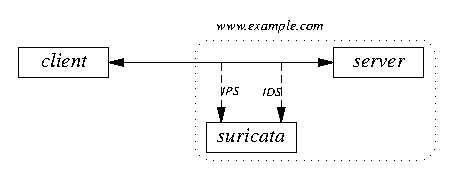
\includegraphics[width=0.6\textwidth]{ids-ips.eps}
\end{figure}

Suricata 提供多种工作模式,主要有 {\cf auto}、{\cf autofp} 以及 {\cf worker} 三种,其中
\begin{itemize}
    \item 三种模式中数据包都是线性处理的,数据包的状态处于不断变化之中,在不同的模块中,对数据包进行不同的切分和处理,最终完成检测和保护功能。
    \item {\cf auto} 和 {\cf autofp} 是类似的,各个模块以线程进行划分,每个模块分别有一个线程对应处理,线程之间以同步的信号量进行通信。数据包都是从一个线程模块转移到另一个线程模块,在数据包转移的过程中,会对数据包进行不同的处理。所不同的是 {\cf autofp} 提供了负载均衡功能({\ef auto flow pinned load balancing})。
    \item {\cf worker} 模式和前两者不同,它在同一个线程中完成对所有模块的处理,也即流水线上的所有模块都运行于同一个线程中,而在整个 Suricata 内部,有多个这样的流水线,分别处理各自的数据,线程彼此之间没有数据包传递。
\end{itemize}

Suricata 中单个流水线的处理流程为:

\begin{figure}[ht!]
    \centering
    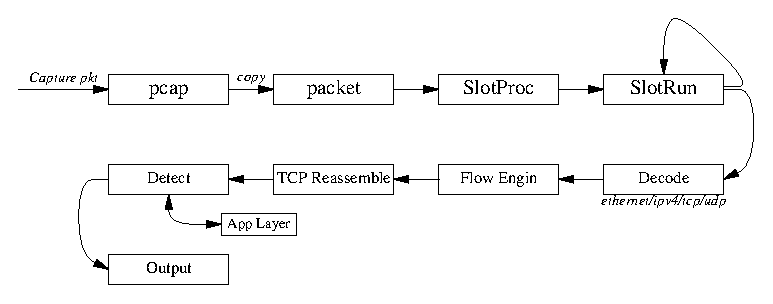
\includegraphics[width=0.9\textwidth]{suricata.eps}
\end{figure}

下面以 Mysql 协议为例,详细说明如何在 Suricata 框架中添加自定义协议识别、关键字识别、日志模块等内容。

\section{在 Suricata 中加入 MySQL 协议检测}
在 Suricata 中添加 MySQL 协议的的检测,只需要在应用层({\ef App Layer})增加相应的模块即可。具体分为以下几个步骤:

\begin{enumerate}
    \item 增加协议号。
    \item 加入新的模块,将其命名为 {\cf app-layer-mysql.c}。
    \item 增加编译设置,将新加入的模块编译进 Suricata 中。
\end{enumerate}

在头文件 {\ff src/app-layer-protos.h} 的枚举 {\cf AppProto} 中加入一个新的成员 {\cf ALPROTO\_MYSQL} 即完成了协议号添加, 下面具体说明一下新模块的编写。

在 Suricata 中,所有的协议注册都是在 {\ff src/app-layer-parser.c} 模块中完成的,所有的第三方协议模块必须提供一个注册 API 给该模块,以完成其协议注册。在这里,MySQL 的协议支持模块为 {\ff src/app-layer-mysql.[ch]},注册函数为 {\cf RegisterMysqlParsers()}。

\begin{lstlisting}
/* src/app-layer-mysql.c */
void RegisterMysqlParsers(void) {
    ...
}

/* src/app-layer-mysql.h */
void RegisterMysqlParsers(void);
\end{lstlisting}

在 {\cf RegisterMysqlParsers()} 函数中,至少需要做以下几个步骤:

\begin{itemize}
    \item 调用 {\cf AppLayerProtoDetectConfProtoDetectionEnabled} 测检测协议支持是否启用。
    \item 调用 {\cf AppLayerProtoDetectRegisterProtocol} 添加对应用协议的支持。
    \item 调用 {\cf AppLayerProtoDetectPPParseConfPorts} 函数将对应的协议号以及协议检测回调函数注册到 {\ff src/app-layer-parser.c} 模块中。
    \item 调用 {\cf AppLayerParserRegisterParser} 注册(2 个)协议解析函数。
    \item 调用 {\cf AppLayerParserRegisterStateFuncs} 注册两个内存管理函数(alloc/free),用以管理协议状态对象的内存。
\end{itemize}

这里需要注意以下协议检测函数的注册,在 Suricata 中,有两类协议注册函数,一类为 ``带关键字的协议识别注册函数 '' 以及 ``不带关键字的协议识别注册函数''。对前者而言,比如在 HTTP 协议中,常见的关键字有 {\cf GET}、{\cf POST} 等,如果要识别这样的数据包,可调用函数 {\cf AppLayerProtoDetectPMRegisterPatternCS} 或函数 {\cf AppLayerProtoDetectPMRegisterPatternCI};
\footnote{这两者的区别在于是否对关键字的大小写进行区分。}
当某些通信协议没有关键字时,比如 DNS 协议或 MySQL 协议,则使用函数 {\cf AppLayerProtoDetectPPParseConfPorts} 。所不同的是,由于后者并未提供关键字识别,所以需要另行传入一个函数来检测应用层数据流,并且,当该检测函数返回时,将对应的协议号(也即 {\cf ALPROTO\_MYSQL})作为其返回值,否则返回 {\cf ALPROTO\_FAILED},表示数据流和所支持的协议不匹配\footnote{可以通過在 {\ff suricata.yaml} 中增加協議以及端口來匹配发送給服务端的数据,這样更为可靠。}。

除此之外,Suricata 会使用协议模块中一个重要的数据结构,即协议状态对象。在该对象中,你可以设置所需的任何数据,因为它对 Suricata 而言是一个 {\cf void *} 对象。在一个通信的生命周期内,该状态会一直存在,所以你至少可以在其中保存通信的状态信息,以便于通信协议的解析。由于该对象由 Suricata 主框架初始化,所以你需要将该对象的内存管理函数告知 Suricata。

完成代码后,需要将其加入到 Suricata 的编译规则中来,在 {\ff src/Makefile.am} 中,于 {\cf suricata\_SOURCES} 列表中加入新加的代码文件名即可。

对于新加入的代码,Suricata 主框架代码会调用它们,对此需要添加相应的头文件包含。对新加入的应用层模块,需要在 {\ff src/app-layer-parser.c} 的 {\cf AppLayerParserRegisterProtocolParsers} 函数中增加其注册函数的调用。

\section{修改 Suricata 配置文件}
如果要让新的模块可以正常运行,还需要将该模块的配置添加到配置文件中。在 Suricata 的配置文件 {\ff suricata.yaml} 中,在 {\cf app-layer.protocols} 中加入 {\cf mysql}:

\begin{lstlisting}
app-layer:
  protocols:
    mysql:
      enabled: yes
      detection-ports:
        tcp:
          toserver: 3306
\end{lstlisting}

注意,这里指定了具体的协议以及端口,客戶端的数据只有通过 TCP 发送到 3306 端口才能被 MySQL 所註冊的模块捕获,這樣做的好處就是不会遗漏發送給服務器端的數據,即使該數據包的格式可能不對。

\section{在 Surcata 中增加关键字识别}
关键字的识别主要用于 detect 模块对数据报文的分析。这些关键字通常都配置在规则文件中,在规则文件中,可以针对关键字上发生的动作做不同的行为选择,比如,如果定义了与 MySQL 相关的规则识别,当有用户以 {\cf root} 用户名登陆数据库时,则处罚 detect 模块中的一个警告信息,其规则大概为

\begin{lstlisting}
alert mysql any any -> any any (msg:"mysql user(root) detected";
	flow:to_server,established; mysql-user:root; sid:2240000; rev:1;)
\end{lstlisting}

其中,{\cf alert} 即 detect 模块的一种行为,其它几种行为有 {\cf pass}、 {\cf reject}、{\cf drop}。后面的 {\cf mysql} 即规则的种类,在 Suricata 中,默认内置了多种规则种类,如 TLS、HTTP、DNS 等等。后面的四个 {\cf any} 即表示一个 socket 连接元素,分别代表源端和目的端的 IP 和端口,箭头 {\cf ->} 表示数据流向。后面 {\cf()} 中的类容就是具体规则的文法表示;此处的 {\cf msg} 就是警告信息最后写入日志文件的字符串,{\cf flow} 表示数据流,此处它有两个属性,一个表述数据流向,一个表述连接已经建立。后面的 {\cf mysql-user} 也是一个即将添加的关键字,它用来承接规则中指定的用户名。后面的 {\cf sid} 表示当前规则的全局 ID,在 Suricata 中,通常会划分一个 ID 区间给特定种类的规则(类似 IP 段划分);最后的 {\cf rev} 应该表示版本,因为规则文件可能时常变迁(根据不同的安全环境),用它来记录一些版本的情况,便于维护。

要使得上面的这条规则生效,可以先在 {\ff rules/} 中增加 {\ff mysql-events.rules} 文件。下面以关键字 {\cf mysql-user} 为例,分析一下如何在 Suricata 中增加新的关键字。

在 {\cf mysql-events.rules} 中,增加上面列出那个示例规则,它表示当用户 {\cf root} 登陆时,记录一条 {\cf alert} 信息到日志文件中,此处的日志信息记录在文件 {\ff log/suricata/fast.log} 中。下面是一个 log 例子:

\begin{lstlisting}[breaklines=true]
01/09/2014-15:34:21.196162  [**] [1:2240001:1] mysql user(root) detected [**] [Classification: (null)] [Priority: 3] {TCP} 192.168.36.131:54107 -> 192.168.37.119:3306
\end{lstlisting}

接下来就是在代码中添加具体的模块,来实关键字的识别。

\section{增加关键字识别的实现}
以增加关键字 {\cf mysql} 以及 {\cf mysql-user} 为例,需要做以下几个工作:
\begin{enumerate}
    \item 增加协议关键字识别,此处指前面的 {\cf mysql} 关键字,它是 MySQL 协议的标识,它之下可以涵盖其它与 MySQL 相关的关键字。
	\item 增加关键字识别模块,此处即各种与 MySQL 相关的关键字。
    \item 在 {\ff src/detect.h} 的枚举中增加一些宏定义,这些宏定义就是各种 MySQL 关键字的索引。
\end{enumerate}

从上一节中可以看到,在动作 {\cf alert} 后面加入了一个 {\cf mysql} 关键字,这就使得该条规则只会匹配 MySQL 的通信数据,而不会干扰其它应用层(如 HTTP)或协议层数据(如 IP 或 TCP)。由于前面已经加入了 MySQL 应用层,所以这里使用 {\cf mysql} 作为匹配 MySQL 关键字的协议识别,注意,如果要修改协议识别(如将其改成 {\cf mysql-4.1}),那么在 {\cf RegisterMysqlParsers} 函数中也需要更新,将参数 {\cf proto\_name} 改成相应值。之所以它们之间有强烈的关联,是因为 {\cf app-layer} 模块的初始化先于签名规则的初始化,所以,后者能在 {\cf app-layer} 模块中找到与关键字匹配的协议。

\begin{quote}
    此处可以视作模块间的耦合,如果在 detect 模块也加入一种识别,而不借助 app-layer 模块的关键字,更易于理解和实现。
\end{quote}

下一步就是增加关键字识别模块 {\ff src/detect-mysql-keywords.[ch]},该子模块被 Detect 模块调用,以检测规则签名中的规则是否匹配。

若在该子模块中增加关键字 {\cf mysql-user} 的识别和检测,需要做以下几个步骤:

\begin{enumerate}
	\item 编写注册函数 {\cf DetectMysqlKeywordsRegister},在其中中追加几个回调函数:
	\begin{enumerate}
		\item 关键字 {\cf mysql-user} 的设置函数:{\cf DetectMysqlUserSetup()}
		\item 匹配关键字 {\cf mysql-user} 的函数:{\cf DetectMysqlUserALMatch()},其中 {\cf AL} 指应用层。
		\item 如果关键字值的匹配过程中需要分配新的对象,则另需注册一个该对象的资源管理函数,用于释放内存。在 {\cf mysql-user} 关键字中,该函数为 {\cf DetectMysqlUserFree()}。
	\end{enumerate}
    \item 在 detect 模块的 {\cf SigTableSetup} 函数中增加对该注册函数的调用。
\end{enumerate}

函数 {\cf DetectMysqlKeywordsRegister} 是这样子的:

\begin{lstlisting}
void DetectMysqlKeywordsRegister(void) {
	sigmatch_table[DETECT_AL_MYSQL_USER].name = "mysql-user";
	sigmatch_table[DETECT_AL_MYSQL_USER].desc = "mysql TBD";
	sigmatch_table[DETECT_AL_MYSQL_USER].url = "mysql TBD";
	sigmatch_table[DETECT_AL_MYSQL_USER].Match = NULL;
	sigmatch_table[DETECT_AL_MYSQL_USER].AppLayerMatch = DetectMysqlUserALMatch;
	sigmatch_table[DETECT_AL_MYSQL_USER].alproto = ALPROTO_MYSQL; 
	sigmatch_table[DETECT_AL_MYSQL_USER].Setup = DetectMysqlUserSetup;
	sigmatch_table[DETECT_AL_MYSQL_USER].Free = DetectMysqlUserFree;
	sigmatch_table[DETECT_AL_MYSQL_USER].RegisterTests = NULL;
	sigmatch_table[DETECT_AL_MYSQL_USER].flags |= SIGMATCH_PAYLOAD;

	/* ... you can add more keywords here */
}
\end{lstlisting}

这里要注意的是,匹配的回调函数有两个,一个是 {\cf Match},一个是 {\cf AppLayerMatch},前者主要用于协议层,如校验和检查,后者用于应用层。这两个回调函数的参数很不同,直接影响匹配的结果。

从上面的代码中可以看到,主要的字段是 {\cf name},将其设置成 {\cf mysql-user},它就是关键字的名称;其中 {\cf desc} 和 {\cf url} 主要做日志使用,便于调试。{\cf alproto} 即之前应用层中注册的宏 {\cf ALPROTO\_MYSQL},最后在 {\cf flags} 上追加属性 {\cf SIGMATCH\_PAYLOAD},便于 Detect 模块的识别。

这里的几个回调函数都是由 Detect 模块来调用。{\cf DetectMysqlUserSetup} 用来设置关键字,它会新建一个 {\cf DetectMysqlUser} 对象,该对象由具体的关键字逻辑定义,此处只是将关键字 {\cf mysql-user} 作为其唯一的字段,在分析规则文件中的规则时,会将关键字传入该函数。对象新建完以后,它以 {\cf void *} 的形式被加入到 {\cf SigMatch} 对象中,作为关键字 {\cf mysql-user} 检测的辅助对象({\cf ctx})。

函数 {\cf DetectMysqlUserFree} 用来释放 {\cf DetectMysqlUser} 对象。

函数 {\cf DetectMysqlUserALMatch} 就是具体的匹配函数,它带入的参数非常之多,常常只需要用几个行了。此处简单地将 {\cf DetectMysqlUser} 中的字段与 {\cf alstate} 中的用户名做一下对比即可直到是否匹配该规则。同时此处会代入 {\cf Signature} 对象,其中有该条规则的动作字段,可以将其设置在 {\cf MysqlTransaction} 中,用于将具体的动作记录到日志文件中。

接下来在 {\ff src/detect.h} 中增加宏定义 {\cf DETECT\_AL\_MYSQL\_USER}\footnote{注意,如果增加其它关键字,则需要增加新的宏定义。}。在 {\ff src/detect.c} 中增加 MySQL 关键字模块的头文件包含:

\begin{lstlisting}
#include "detect-mysql-keywords.h"
\end{lstlisting}

然后在 {\ff src/Makefile.am} 的 {\cf suricata\_SOURCE} 中增加新模块编译规则即可。

\section{增加 Json 输出模块}
在现有的 Suricata 中,log 模块依旧使用其自定义的格式记录,但是 event 时间则采用 JSON 格式记录。本节只涉及 event 相关的 JSON 记录。在 Suricata 中,以文件 {\ff output-json-xxx.[ch]} 命名的模块有 DNS、HTTP、SSH、TLS 等。此处仿照其实现,以 MySQL 协议为例,说明一下如何在 Suricata 中添加 JSON 的日志输出功能。

\section{Suricata 开发过程中碰到的疑难问题}\label{sec:dev-problems}
在 Suricata 的日常开发中,碰到一些比较难的问题,这些问题需要深挖 Suricata 的底层实现。现将其一一列举出来,以备日后查看。

\subsection{Suricata 只能将小部分的 TNS 协议数据包送到应用协议层}
具体的表现症状就是当抓取登录数据包时,只有前面几个数据包被抓取到了,后面的数据包全部没有上浮到应用层,导致应用层无法解析数据包。但是登陆的过程以及后续的 SQL 执行都能正常进行,这表明数据确实从 Suricata 中穿过去了,但是没有上报到应用层。

一步步跟踪发现,数据没有到达应用层是因为从到应用层中间的处理应为某种原因中断了,从而数据没有上报。具体的地点是:

在函数 {\cf StreamTcpReassembleInlineAppLayer} 的 {\cf for (; seg != NULL;)}中,有如下代码

\begin{lstlisting}[stepnumber=1,numbersep=8pt,numberstyle=\tiny\color{blue},numbers=left]
...
for (; seg != NULL;) {
    if (p->flow->flags & FLOW_NO_APPLAYER_INSPECTION) {
        if (seg->flags & SEGMENTTCP_FLAG_RAW_PROCESSED) {
        SCLogDebug("removing seg %p seq %"PRIu32
            " len %"PRIu16"", seg, seg->seq, seg->payload_len);

        TcpSegment *next_seg = seg->next;
        StreamTcpRemoveSegmentFromStream(stream, seg);
        StreamTcpSegmentReturntoPool(seg);
        seg = next_seg;
        continue;
    } else {
        break;
    }
}
...
\end{lstlisting}

其中,第三行的条件成立,但是第四行不成立,导致退出当前的 {\cf for} 循环,但是这个 {\cf for} 循环是非常重要的,其中涉及将 {\cf Packet} 对象中的数据拷贝出来,并调用 {\cf AppLayerHandleTCPData} 进入应用层处理。{\cf for} 循环退出之后,函数 {\cf StreamTcpReassembleInlineAppLayer} 基本退出,导致这个数据包不能进入应用层处理。

发现现场之后,可以进一步挖掘,为何会进入第三行这个 {\cf if} 语句,宏 {\cf FLOW\_NO\_APPLAYER\_INSPECTION} 是在什么时候设置上去的?通过 {\cmdf grep} 一下源码树,发现在文件 {\ff src/flow.h} 中定义了一个函数 {\cf FlowSetSessionNoApplayerInspectionFlag},就是通过它来设置这个标志位的。接下来再 {\cmdf grep} 这个函数,发现了如下一些地方

\begin{lstlisting}
src/app-layer.c:244:         FlowSetSessionNoApplayerInspectionFlag(f);
src/app-layer.c:273:         FlowSetSessionNoApplayerInspectionFlag(f);
src/app-layer.c:327:         FlowSetSessionNoApplayerInspectionFlag(f);
src/app-layer.c:351:         FlowSetSessionNoApplayerInspectionFlag(f);
src/app-layer-parser.c:835:  FlowSetSessionNoApplayerInspectionFlag(f);
src/app-layer-parser.c:862:  FlowSetSessionNoApplayerInspectionFlag(f);
src/detect.c:11060:          FlowSetSessionNoApplayerInspectionFlag(p2->flow);
src/detect.c:11243:          FlowSetSessionNoApplayerInspectionFlag(p2->flow);
src/flow.h:426:static inline void FlowSetSessionNoApplayerInspectionFlag(Flow *);
src/flow.h:494:static inline void FlowSetSessionNoApplayerInspectionFlag(Flow *f) {
src/stream-tcp.c:4201:       FlowSetSessionNoApplayerInspectionFlag(p->flow);
\end{lstlisting}

%由于此时代码逻辑尚未进入应用层,所以可以肯定这个标志位要么在 detect 模块谁定,要么在 stream TCP 模块设定。

在该函数处设置断点,第一次触发该断点的调用栈为

\begin{lstlisting}
#0  FlowSetSessionNoApplayerInspectionFlag (f=0x8ef76a8) at flow.h:495
#1  0x080a561c in AppLayerParserParse (alp_tctx=0xb6512c20, f=0x8ef76a8, alproto=14, flags=4 '\004', input=0xb6e8d5bc "", input_len=1448) at app-layer-parser.c:862
#2  0x0805e771 in AppLayerHandleTCPData (tv=0x9125f20, ra_ctx=0xb6512af8, p=0x8d3e5c0, f=0x8ef76a8, ssn=0xb6595160, stream=0xb65951a0, data=0xb6e8d5bc "", data_len=1448, flags=4 '\004') at app-layer.c:360
#3  0x082ce657 in StreamTcpReassembleInlineAppLayer (tv=0x9125f20, ra_ctx=0xb6512af8, ssn=0xb6595160, stream=0xb65951a0, p=0x8d3e5c0) at stream-tcp-reassemble.c:2383
#4  0x082d7afd in StreamTcpReassembleHandleSegment (tv=0x9125f20, ra_ctx=0xb6512af8, ssn=0xb6595160, stream=0xb65951a0, p=0x8d3e5c0, pq=0xb65126ec) at stream-tcp-reassemble.c:3632
#5  0x08296ab9 in HandleEstablishedPacketToServer (tv=0x9125f20, ssn=0xb6595160, p=0x8d3e5c0, stt=0xb65126e0, pq=0xb65126ec) at stream-tcp.c:1969
#6  0x0829aed3 in StreamTcpPacketStateEstablished (tv=0x9125f20, p=0x8d3e5c0, stt=0xb65126e0, ssn=0xb6595160, pq=0xb65126ec) at stream-tcp.c:2323
#7  0x082b4426 in StreamTcpPacket (tv=0x9125f20, p=0x8d3e5c0, stt=0xb65126e0, pq=0x9126188) at stream-tcp.c:4243
#8  0x082b5588 in StreamTcp (tv=0x9125f20, p=0x8d3e5c0, data=0xb65126e0, pq=0x9126188, postpq=0x0) at stream-tcp.c:4485
#9  0x082ef0a4 in TmThreadsSlotVarRun (tv=0x9125f20, p=0x8d3e5c0, slot=0x9126088) at tm-threads.c:559
#10 0x08276651 in TmThreadsSlotProcessPkt (tv=0x9125f20, s=0x9126088, p=0x8d3e5c0) at tm-threads.h:142
#11 0x08277f0a in NFQCallBack (qh=0xb6500620, nfmsg=0xb6500648, nfa=0xb6e908ac, data=0x8430000 <nfq_t>) at source-nfq.c:524
...
\end{lstlisting}

从 {\cf \#6} 开始,从此处建立连接,开始接收数据包,到 {\cf \#5} 中处理数据包,在 {\cf \#4} 中重组接收到的数据包,进入 {\cf \#3},在函数 {\cf StreamTcpReassembleInlineAppLayer} 中进入 {\cf \#2},注意,此时进入了 app-layer 逻辑层。然后进一步进入函数 {\cf AppLayerParserParse},最终在该函数中调用 {\cf FlowSetSessionNoApplayerInspectionFlag}。之所以调用该函数,是因为某个 {\cf goto} 语句发现了某个条件不符合,这几个条件是

\begin{itemize}
    \item 发现了 stream gap
    \item {\cf AppLayerParserState} 对象分配失败
    \item app-layer 的 state 对象分配失败
    \item app-layer 的 parser 函数执行失败
\end{itemize}

\chapter{Suricata 预研 Demo}\label{chap:demo}

\section{主要内容}

\begin{itemize}
    \item 环境搭建
    \item 协议分析(在前面的章节中,此处不表)
    \item 效果展示(IDS/IPS)
\end{itemize}

\section{网络结构}
Suricata 和数据库客户端均位于同一台机器。数据库服务器位于 182 以及 194。其网络结构如图所示:

\begin{tikzpicture}
    %\draw[help lines](0,0) grid(14,3);

    % 两个客户端工具
    \node [above] at (1.5, 1.75) {\cf mysql\_cli};
    \draw (0.5, 1.75) rectangle (2.5,2.25);
    \node [below] at (1.5, 1.25) {\cf oracle\_cli};
    \draw (0.5, 0.75) rectangle (2.5,1.25);

    % 宿主机
    \draw [rounded corners, purple, dashed](0,0) rectangle (7,3);
    \node [below] at (3.5, 0.5) {\cf 宿主机器(174)};

    % suricata
    \draw (4.5, 1) rectangle (6.5,2);
    \node at (5.5, 1.5) {\cf suricata};
    
    % db server
    \node [above] at (10.5, 1.75) {\cf mysql\_srv(182)};
    \draw (9, 1.75) rectangle (12,2.25);
    \node [below] at (10.5, 1.25) {\cf oracle\_srv(194)};
    \draw (9, 0.75) rectangle (12,1.25);

    % lines
    \draw[->,  teal] (1.5, 2.25) to [out=10,in=170] (10.5, 2.25);
    \draw[->,  teal] (1.5, 2.25) to [out=10, in=150] (5.5, 2);
    \draw[->,  teal] (1.5, 0.75) to [out=350,in=190] (10.5, 0.75);
    \draw[->,  teal] (1.5, 0.75) to [out=350, in=210] (5.5, 1);
    
    \draw[->,  blue] (2.5, 2) -- (4.5, 1.75);
    \draw[->,  blue] (6.5, 1.75) -- (9, 2);
    \draw[->,  blue] (2.5, 1) -- (4.5, 1.25);
    \draw[->,  blue] (6.5, 1.25) -- (9, 1);

    \draw[->, blue] (10,3.25) -- (11, 3.25);
    \node [right] at (11, 3.25) {\cf \scriptsize NFQ IPS 模式};
    \draw[->,  teal] (10,2.75) -- (11, 2.75);
    \node [right] at (11, 2.75) {\cf \scriptsize PCAP IDS 模式};
\end{tikzpicture}

\section{Suricata IDS/IPS 对现有数据库协议支持的展示}
目前对 MySQL 的协议以及基本支持,能获取对应的 SQL 语句以及更详细的信息。对 Oracle 11g 数据库而言,目前可以拿到其基本的 SQL 语句信息,其它更深入的信息(session 管理、返回的数据分析)尚不能获取。

\subsection{IDS 功能演示}

以命令 {\cf ./suricata r -c yaml/demo.yaml -i eth1} 启动 IDS 模式的 Suricata,此处使用 eth1 作为嗅探网卡。

对 Oracle 以及 MySQL 数据库而言,分别对应如下两条检测规则:

\begin{lstlisting}[language=python]
alert `\hl{red}{oracle11g}` any any -> any any (msg:"oracle user(coanor) detected";
    flow:to_server,established; `\hl{blue}{oracle11g-user}`:coanor; sid:2250000; rev:1;)
alert oracle11g any any -> any any (msg:"oracle database(orcl11g) detected";
    flow:to_server,established; `\hl{blue}{oracle11g-sid}`:orcl11g; sid:2250001; rev:1;)
\end{lstlisting}

\begin{lstlisting}[language=python]
alert `\hl{red}{mysql}` any any -> any any (msg:"mysql user(root) detected";
    flow:to_server,established; `\hl{blue}{mysql-user}`:root; sid:2240000; rev:1;)
alert mysql any any -> any any (msg:"mysql database(aap_log) detected";
    flow:to_server,established; `\hl{blue}{mysql-database}`:aap_log; sid:2240001; rev:1;)
\end{lstlisting}

对这两条规则而言,如果满足其检测条件,就会在 {\ff fast.log} 文件中记录相应的 alert 信息。同时,在 MySQL 以及 Oracle 的 JSON 文件日志中,也会记录这一行为(JSON 文件中的 {\cf action} 字段)。对其它几种行为而言,分别更改前面的 {\cf alert} 即可。

alert 日志在常规的 JSON 日志中为:

\begin{lstlisting}
{
    "timestamp":"2014-06-03T10:09:54.203021",
    "event_type":"oracle11g",
    "src_ip":"192.168.37.174",
    "src_port":45827,
    "dest_ip":"192.168.37.194",
    "dest_port":1521,
    "proto":"TCP",
    "oracle11g":{"user":"coanor",
        "db_name":"orcl11g",
        `\hl{blue}{"action":"ALERT"}`,
        "meta_info":{"sql":null, "cmd":"unkonw"}
    }
}
\end{lstlisting}

常规的 SQL 日志输出示例为:

\begin{lstlisting}
{
    "timestamp":"2014-06-03T10:12:30.534439",
    "event_type":"oracle11g",
    "src_ip":"192.168.37.174",
    "src_port":45827,
    "dest_ip":"192.168.37.194",
    "dest_port":1521,
    "proto":"TCP",
    "oracle11g":{
        "user":"coanor",
        "db_name":"orcl11g",
        "action":"UNKNOWN",
        "meta_info":{
            "sql":`\hl{blue}{"insert into employee (EMPLOYEE\_ID, MANAGER\_ID,
                   FIRST\_NAME, LAST\_NAME, TITLE, SALARY)
                   values( 1 , 0 , 'James' , 'Smith' , 'CEO', 800000)"}`,
            "cmd":"query"
        }
    }
}
\end{lstlisting}

在 {\ff fast.log} 文件中的示例为

\begin{lstlisting}
06/03/2014-13:38:41.827922  [**] [1:2250000:1] oracle user(coanor) detected [**]
    [Classification: (null)] [Priority: 3] {TCP} 192.168.37.174:46697 -> 192.168.37.194:1521
\end{lstlisting}

\subsection{IPS 功能演示}

设置如下 iptables 规则后,再启动 Suricata {\cf ./suricata -c yaml/demo.yaml -q 0}。

\begin{lstlisting}
sudo iptables -A INPUT -j NFQUEUE
sudo iptables -A OUTPUT -j NFQUEUE

# 允许 SSH 访问,便于调试
sudo iptables -I INPUT -p tcp -m tcp --dport 22 -j ACCEPT
sudo iptables -I OUTPUT -p tcp -m tcp --sport 22 -j ACCEPT
\end{lstlisting}

连接建立后,显示的结果数据和 IDS 模式下的一致。

%\include{reading-sc}

\end{document}
